% ======================================================== %
% Przeczytaj plik amuthesis-doc.pdf, aby poznać opcje      %
% klasy `amuthesis`                                        %
% ======================================================== %
\documentclass[oneside,polski,logo]{amuthesis}

% Zdefiniuj kodowanie pliku źródłowego (domyślnie utf8)
\usepackage[utf8]{inputenc}
\usepackage{tikz}
% ======================================================== %
% Dane autora i pracy                                      %
% ======================================================== %

% --- Autor pracy
\author{Bohdan Bondar, Marcin Jałoński, Aleksander Mendoza-Drosik}
% --- Numer albumu
\album{sS432778,s434701,s434749}
% --- Tytuł pracy (w języku polskim i angielskim)
\titlePL{Solomonoff - kompilator transduktorów skończenie stanowych}
\titleEN{Solomonoff - Finite state tranducer compiler}
% --- Typ pracy (inżynierska, licencjacka, magisterska)
\type{inżynierska}
% --- Wydział (wykaz skrótów):
% --- --- WA    --- Wydział Anglistyki
% --- --- WB    --- Wydział Biologii
% --- --- WCh   --- Wydział Chemii
% --- --- WFPiK --- Wydział Filologii Polskiej i Klasycznej
% --- --- WF    --- Wydział Fizyki
% --- --- WH    --- Wydział Historyczny
% --- --- WMiI  --- Wydział Matematyki i Informatyki
% --- --- WNGiG --- Wydział Nauk Geograficznych i Geologicznych
% --- --- WNPiD --- Wydział Nauk Politycznych i Dziennikarstwa
% --- --- WNS   --- Wydział Nauk Społecznych
% --- --- WN    --- Wydział Neofilologii
% --- --- WPAK  --- Wydział Pedagogiczno-Artystyczny w Kaliszu
% --- --- WPiA  --- Wydział Prawa i Administracji
% --- --- WSE   --- Wydział Studiów Edukacyjnych
% --- --- WT    --- Wydział Teologiczny
% --- --- IKE   --- Instytut Kultury Europejskiej w Gnieźnie
\faculty{WMiI}
% --- Kierunek (w mianowniku)
\field{informatyka}
% --- Specjalność (w formie mianownikowej)
% --- (ustaw puste, jeśli bez specjalności)
\specialty{}
% --- Promotor (w dopełniaczu)
\supervisor{dr Bartłomieja Przybylskiego}
% --- Data złożenia pracy (Miasto, miesiąc rok)
\date{Poznań, luty 2021}

% --- Płeć autora (M/K)
\stsex{M/M/M}
% --- Zgoda na udostępnienie pracy w czytelni (TAK/NIE)
\stread{TAK/TAK/TAK}
% --- Zgoda na udostępnienie pracy w zakresie ochrony (TAK/NIE)
\stprotect{TAK/TAK/TAK}
% --- Data podpisania oświadczenia (Miasto, data)
\stdate{Poznań, \today{} r.}

% ======================================================== %
% Dodatkowe pakiety wykorzystywane w pracy                 %
% ======================================================== %

\usepackage{lipsum}

% ======================================================== %
% Zasadnicza część dokumentu                               %
% ======================================================== %

\begin{document}

% Strona tytułowa
\maketitle
% Oświadczenie
\makestatement

% Blok abstraktu w języku polskim
\begin{streszczenie}



\paragraph{Słowa kluczowe:} klasa
\end{streszczenie}

% Blok abstraktu w języku angielskim
\begin{abstract}
\lipsum[2]

\paragraph{Keywords:} klasa
\end{abstract}

% Opcjonalny blok dedykacji
\begin{dedykacja}
Tu możesz umieścić swoją dedykację.
\end{dedykacja}

% Spis treści
\tableofcontents

% ======================================================== %
% Właściwa część pracy                                     %
% ======================================================== %

\chapter{Introduction}


This project focuses on research in the field of automata theory and inductive inference.  The main product of our work is the "Solomonoff" regular expression compiler for finite state transducers. Plenty of research has gone into development of the theory behind this system. As a result the transducers contain several features not known before. 

The most innovative achievements is the lexicographic arctic semiring of weights\cite{MendozaDrosik2020MultitapeAA}, specialized adaptation of Glushkov's construction for subsequential transducers and the most significant flagship feature - built-in support for inductive inference and machine learning of transducers. Thanks to the cooperation with LearnLib and Dortmund University, Solomonoff supports learning algorithms such as RPNI and several of it's  derivatives. We contributed to LearnLib a specialized algorithm for inference of transducers. In particular we implemented OSTIA for efficient learning of deterministic transducers. For nondeterministic ones we developed our own OFTIA algorithm, which was not known before. Additionally we provide an alternative version of OSTIA extended with heuristic search.

All those features together make Solomonoff a unique library that stands out from the alternatives. We support most of the features of UNIX regexes. It's possible to achieve mechanics equivalent to those of look-aheads and look-behinds, which is unusual for automata-based regex engine. The key to Solomonoff 's expressiveness is the possibility of emulating look-aheads with careful placement of transducer outputs. As a result Solomonoff can compete and  do much more than existing projects such as RE2 developed by Google, BRICKS automata developed at Aarhus University or even to certain extent with Pearl/Java based regular expression engines. Another, much stronger competitor for Solomonoff is the OpenFST project developed by Google in collaboration with University of New York. There is a vast intersection of features supported by both libraries, although OpenFST puts heavy emphasis on probabilistic transducers, whereas Solomonoff has better support for formal verification and machine learning. Our project won't be a replacement for OpenFST in the foreseeable future but there are areas where Solomonoff performs better. This is particularly palpable in efficiency as indicated by several of our benchmarks.

Unlike most other automata libraries, Solomonoff's development focuses on the compiler and regular expressions instead of library API. Everything can be achieved without writing Java code. Such approach also allows the developers for much greater flexibility, because the internal implementation can be drastically changed at any time, without breaking existing regular expressions. The public API is minimalist. As a result backwards-compatibility is rarely an issue.  

Another feature of Solomonoff, which is uncommon among regular expression engines is its integrated build system. Our compiler was designed for large codebases consisting of multiple files with dependencies. Thrax is the only alternative that does have a "build system" but it's very primitive and relies on generating Makefiles. Solomonoff has a well integrated tool that assembles large projects, detects cyclic dependencies, allows for parallel compilation and performs additional code optimisations. 


Our project strives to make automata as easy to use and accessible to mass audiences as possible. For this reason we developed a website with online playground where visitors could test Solomonoff and experiment without any setup required. The backend technology we used is Spring Boot, because it allowed for convenient integration with existing API in Java. The website provides downloads of prepackaged JAR files as well as syntax highlighting rules for several popular text editors. 



To allow for easy experimentation and to lower the barrier of entry, Solomonoff comes with interactive shell. It allows for efficient and convenient work with the compiler from command-line interface, where local changes can be hot-swapped and reloaded on live compiler session. Developers could then test their regular expressions without the need to fully recompile their project. 

The REPL console can be easily and painlessly explored without local installation. The website comes with online version of compiler, which can be accessed from any major browser (IE not supported). Most of the command-line features can be used in the online environment, with a few exceptions of features specific only to locally-running instances (especially those allowing for saving and reading files). 

The online interface can serve as a user-friendly playground for newcomers. It is not meant to be a replacement for locally running compiler. Due to the necessity of communicating with backend server and limited computational resources shared among possibly large number of users, the online REPL has major performance limitations. The command-line interface has been designed and optimised with the purpose of providing high efficiency for codebases containing thousands of lines. It supports parallel compilation and caching of previously compiled units. 

Developers have the ability to modularise their projects. Precompiled automata can ve stored and loaded from packages. The build-system is capable of resolving dependencies.



\chapter{Transducers}


\begin{abstract}
%\boldmath
 Glushkov's construction has many interesting properties and they become even more evident when applied to transducers. This article strives to show the vast range of possible extensions and optimisations for this algorithm.  Special flavour of regular expressions is introduced, which can be efficiently converted to $\epsilon$-free functional subsequential weighted finite state transducers. Produced automata are very compact, as they contain only one state for each symbol (from input alphabet) of original expression and only one transition for each range of symbols, no matter how large. Such compactified ranges of transitions allow for efficient binary search lookup during automaton evaluation. All the methods and algorithms presented here were used to implement open-source compiler of regular expressions for multitape transducers. 
\end{abstract}
% IEEEtran.cls defaults to using nonbold math in the Abstract.
% This preserves the distinction between vectors and scalars. However,
% if the journal you are submitting to favors bold math in the abstract,
% then you can use LaTeX's standard command \boldmath at the very start
% of the abstract to achieve this. Many IEEE journals frown on math
% in the abstract anyway.


 are not many open source solutions available for working with transducers. The most significant and widely used library is OpenFst. Their approach is based on theory of weighted automata\cite{MOHRI3}\cite{DROSTE}\cite{DROSTE2}. Here we propose an alternative approach founded on lexicographic transducers \cite{MendozaDrosik2020MultitapeAA} and Glushkov's algorithm \cite{GLUSHKOV}.


Let $W$ be some set of weight symbols. The free monoid $W^*$ will be out set of weight strings. We assume there is some lexicographic order defined as
\[
b_1w_1 > b_2w_2 \iff w_1 > w_2 \mbox{ or }( w_1=w_2\mbox{ and } b_1 > b_2) \\
\]
where $w_1,w_1\in W$ and $b_1,b_2\in W^*$.  The order is defined only on strings of equal lengths.
Let $\Sigma$ be the input alphabet, $\Sigma^*$ is the monoid of input strings and $D$ is the monoid of output strings.  Lexicographic transducer is defined as tuple $(Q,I,W,\Sigma,D,\delta,\tau)$ where $Q$ is some finite set of states, $I$ is the set of initial states, $\tau$ is a state output (partial) function $Q\rightarrow D \times W$ and lastly $\delta$ represents transitions of the form $\delta \subset Q \times W \times \Sigma \times D \times Q$.

Thanks to $\tau$, such machines are subsequential \cite{MOHRI}\cite{MOHRI2}\cite{HANSAN}\cite{de_la_higuera}. As an example consider the simple transducer from figure \ref{transducer}. The states $q_0$, $q_1$ and $q_2$ have no output, which can be denoted with $\tau(q_0)=\emptyset$. The only set which does have output is $q_3$. Every time automaton finishes reading input string and reaches $q_3$, it will append $d_0$ to its output and then accept. For instance, on input $\sigma_1\sigma_2$ it will first read $\sigma_1$, produce output $d_0d_4$ and go to state $q_1$, then read $\sigma_2$ and append output $d_3$, go to state $q_3$, finally reaching end of input, appending $d_0$ and accepting. The total output would be $d_0d_4d_3d_0$. Note that the automaton is nondeterministic, as it could take alternative route passing through $q_2$ and producing $d_3d_0$. In such scenarios weights are used to disambiguate output. The first route produces weight string $w_2w_3w_1$, while the second produces $w_3w_2w_1$. According to our definition of lexicographic order we have $w_2w_3w_1 > w_3w_2w_1$ (assuming that $w_3>w_2$). Throughout this article we will consider smaller weights to be "better". Hence the automaton should choose $d_3d_0$ as the definitive output for input $\sigma_1\sigma_2$. There might be situations in which two different routes have the exact same (equally highest) weight while also producing different outputs. In such cases, the automaton is ambiguous and produces multiple outputs for one input.


% needed in second column of first page if using \IAENGpubid
%\IAENGpubidadjcol

\section{Expressive power}

There are some remarks to be made about lexicographic transducers.  They recognize relations on languages, unlike "plain" finite state automata (FSA) which recognize languages. If $M$ is some transducer, then we denote its recognized relation with $\mathcal{L}(M)$. Those relations are subsets of $\Sigma^*\times D$. The set of strings $\Sigma^*$ accepted by $M$ must be a regular language (indeed, if we erased output labels, we would as a result obtain FSA). The weights are erasable \cite{MendozaDrosik2020MultitapeAA}  in the sense that, give any lexicographic transducer we can always build an equivalent automaton without weighted transitions. If we didn't have $\tau$, the only output possible to be expressed for empty input would be an empty string as well. With $\tau$ we can express pairs like $(\epsilon,d)\in\mathcal{L}$ where $d\ne\epsilon$.  

The transducers can return at most finitely many outputs for any given input (see \textit{infinite superposition}\cite{MendozaDrosik2020MultitapeAA}). If we allowed for $\epsilon$-transitions (transitions that have $\epsilon$ as input label) we could build $\epsilon$-cycles and produce infinitely many outputs. However, automata that do so are not very interesting from practical point of view. Therefore we shall focus only on functional transducers, that is those which produce at most one output. If automaton does not have any $\epsilon$-cycles and is functional, then it's possible to erase all $\epsilon$-transitions (note that it would not be possible without $\tau$, because $\epsilon$-transitions allow for producing output given empty input). Therefore $\epsilon$-transitions don't increase power of functional transducers.

We say that transducer has \textbf{conflicting states} $q_1$ and $q_2$ if it's possible to reach both of them simultaneously (there are two possible routes with the same inputs and weights) given some input $\sigma$ and there is some another state $q_3$ to which both of those states can transition over the same input symbol $\sigma_i$. Alternatively, there might be no third state $q_3$, but instead both $q_1$ and $q_2$ have non-empty $\tau$ output (so $\tau$ can in a sense be treated like $q_3$). We say that transitions $(q_1,\sigma_i,w,d,q_3)$ and $(q_2,\sigma_i,w',d,q_3)$  are \textbf{weight-conflicting} if they have equal weights $w=w'$.  For instance in figure \ref{transducer} the states $q_1$ and $q_2$ are indeed conflicting because they both transition to $q_3$ over $\sigma_2$ but their transitions are not weight conflicting. It can be shown that transducers without weight-conflicting  transitions are functional. Moreover, if a transducer is functional but contains weight-conflicting transitions, then the weights can be reassigned in such a way that eliminates all conflicts \cite{MendozaDrosik2020MultitapeAA}. The only requirement is that there are enough symbols in $W$ (for instance, if $W$ had only one symbol, then all transitions of conflicting states would always be weight-conflicting). If there are at least as many weight symbols as there are states $\vert W \vert = \vert Q \vert$, then every functional transducer on $\vert W \vert$ states can be built without weight-conflicting transitions. For convenience we can assume that $W=\mathbb{N}$, but in practice all algorithms presented here will work with bounded $W$. Hence transducers without weight-conflicting transitions are equivalent in power to functional transducers. This is important because by searching for weight-conflicting transitions we can efficiently test whether transducer is functional or not.

\section{Ranged automata}


\begin{figure}[!t]
	\centering
	\includegraphics[width=9cm]{transducer} 
	\caption{Example of lexicographic transducer. State $q_0$ is initial. State $q_3$ in accepting, in the sense that $\tau(q_3)=(w_1,d_0)$. The remaining states have state output $\emptyset$.}
	\label{transducer}
\end{figure}

Often when implementing automata the algorithm behind $\delta$ function needs to efficiently find the right transition for a given $\sigma$ symbol. It's beneficial to optimise UNIX-style ranges like \texttt{[0-9]} or \texttt{[a-z]} as they arise often in practical settings. Even the \texttt{.} wildcard can be treated as one large range spanning entire $\Sigma$. If the alphabet is large (like ASCII or UNICODE), then checking every one of them in a loop is not feasible. A significant improvement can be made by only checking two inequalities like $\sigma_1\le x \le \sigma_{10}$, instead of large number of equalities. The current paper presents a way in which simplified model of $(\mathcal{S},k)$-automata\cite{MEER}\cite{Gandhi}, can be used to obtain major improvements. In particular we consider only automata that don't have any registers apart from constant values, that is $k=0$. Therefore we provide a more specialized definition of "ranged automata". 

Let $\Sigma$ be the (not necessarily finite) alphabet of automaton. Let $\chi$ be the set of subsets of $\Sigma$ that we will call \textbf{ranges} of $\Sigma$. Let  $\overline{\chi}$ be  the closure of $\chi$ under countable union and complementation (so it forms a sigma algebra). For instance, imagine that there is total order on $\Sigma$ and  $\chi$ is the set of all intervals in $\Sigma$. Now we want to build an automaton whose transitions are not labelled with symbols from $\Sigma$, but rather with ranges from $\chi$. Union $\chi_0\cup\chi_1$ of two elements from $\chi$ "semantically" corresponds to putting two edges, $(q,\chi_0,q')\in\delta$ (for a moment forget about outputs and weights) and $(q,\chi_1,q')\in\delta$. There is no limitation on the size of $\delta$. It might be countably infinite, hence it's natural that $\overline{\chi}$ should be closed under countable union. Therefore, $\chi$ is the set of allowed transition labels and $\overline{\chi}$ is the set of all possible "semantic" transitions. We could say that $\overline{\chi}$ is discrete if it contains every subset of $\Sigma$. An example of discrete $\overline{\chi}$ would be finite set $\Sigma$ with all UNIX-style ranges \texttt{[$\sigma$-$\sigma'$]} included in $\chi$. 

Another example would be set $\Sigma=\mathbb{R}$ with $\chi$ consisting of all ranges, whose ends are computable real numbers (real number $x$ is computable if the predicate $q<x$ is decidable for all rational numbers $q$). If we also restricted $\delta$ to be a finite set, then we could build effective automata that work with real numbers of arbitrary precision. 



\section{Regular expressions}

Here we describe a flavour of regular expressions specifically extended to interplay with lexicographic transducers and ranged automata. 

Transducers with input $\Sigma^*$ and output $\Gamma^*$ can be seen as FSA working with single input $\Sigma^* \times \Gamma^*$. Therefore we can treat every pair of symbols $(\sigma,\gamma)$ as an atomic formula of regular expressions for transducers. We can use concatenation $(\sigma,\gamma_0)(\epsilon,\gamma_1)$ to represent $(\sigma,\gamma_0\gamma_1)$. It's possible to create ambiguous transducers with unions like  $(\epsilon,\gamma_0)+(\epsilon,\gamma_1)$.  To make notation easier, we will treat every $\sigma$ as $(\sigma,\epsilon)$ and every $\gamma$ as $(\epsilon,\gamma)$. Then instead of writing lengthy $(\sigma,\epsilon)(\epsilon,\gamma)$ we could introduce shortened notation $\sigma:\gamma$. Because we would like to avoid ambiguous transducers we can put restriction that the right side of $:$ should always be a string of $\Gamma^*$ and writing entire formulas (like $\sigma:\gamma_1+\gamma_2^*$) is not allowed. This restriction will later simplify Glushkov's algorithm. 

We define $\mathcal{A}^\Sigma$ to be the set of atomic characters. For instance we could choose $\mathcal{A}^\Sigma=\Sigma\cup\{\epsilon\}$ for FSA/transducers and $\mathcal{A}^\Sigma=\chi$ for ranged automata. 

We call  $RE^{\Sigma:D}$ the set of all regular expression formulas with underlying set of atomic characters $\mathcal{A}^\Sigma$ and allowed output strings $D$. It's possible that $D$ might be a singleton monoid $\{\epsilon \}$ but it should not be empty, because then no element would belong to $\Sigma^* \times D$. By inductive definition, if $\phi$ and $\psi$  are $RE^{ \Sigma:D}$  formulas and $d \in D$, then union $\phi + \psi$, concatenation $\phi \cdot \psi$, Kleene closure $\phi^*$ and output concatenation $\phi : d$ are $RE^{ \Sigma:D}$ formulas as well.  Define $V^{\Sigma:D}:RE^{\Sigma:D} \rightarrow \Sigma^* \times D$ to be the valuation function:  \\
$V^{\Sigma:D}(\phi + \psi) = V^{\Sigma:D}(\phi) \cup V^{\Sigma:D}(\psi)$ \\
$V^{\Sigma:D}(\phi \cdot \psi) = V^{\Sigma:D}(\phi) \cdot  V^{\Sigma:D}(\psi)$ \\
$V^{\Sigma:D}(\phi^*) = (\epsilon,\epsilon) + V^{\Sigma:D}(\phi) + V^{\Sigma:D}(\phi)^2 + ...$ \\
$V^{\Sigma:D}(\phi : d) = V^{\Sigma:D}(\phi)  \cdot (\epsilon,d)$ \\
$V^{\Sigma:D}(a) = a$ where $a\in\mathcal{A}^{\Sigma:D}$ \\
Some notable properties are: \\
$x:y_0 +x:y_1 = x:(y_0+y_1)$ \\
$x:\epsilon+x:y+x:y^2...=x:y^*$ \\
$(x:y_0)(\epsilon:y_1)  = x:(y_0y_1)$\\
$x_0:(y_0y')+x_1:(y_1y') = (x_0:y_0+x_1:y1)\cdot(\epsilon:y')$ \\
$x_0:(y'y_0)+x_1:(y'y_1) = (\epsilon:y')\cdot(x_0:y_0+x_1:y1)$  \\
Therefore we can see that expressive power with and without $:$ is the same. 

It's also possible to extend regular expressions with weights. Let $RE_W^{\Sigma: D}$ be a superset of $RE^{\Sigma: D}$ and $W$ be the set of weight symbols. If $\phi\in RE_W^{\Sigma\rightarrow D}$ and $w_0,w_1\in W$ then $w_0 \phi $ and  $\phi w_1 $ are in $RE_W^{\Sigma\rightarrow D}$. This allows for inserting weight at any place. For instance, the automaton from figure \ref{transducer} could be expressed using \[
((\sigma_1:d_0d_4)w_2(\sigma_2:d_3)w_3+
(\sigma_1:d_3)w_3\sigma_2w_2):d_0
\]
The definition of $V^{\Sigma:D}(\phi w)$ depends largely on $W$ but associativity $(\phi w_1) w_2 = \phi (w_1 + w_2)$ should be preserved, given that $W$ is a multiplicative monoid. This also implies that $w_1 \epsilon w_2 = w_1 w_2$, which is semantically equivalent to the addition $w_1 + w_2$. 

We showed that regular expressions for transducers can be expressed using pairs of symbols $(\sigma,\gamma)$. There is an alternative approach. We can encode both input and output string by interleaving their symbols like $\sigma_1\gamma_1\sigma_2\gamma_2$. Such regular expressions "recognize" relations rather than "generate" them. This approach has one significant problem. We have to keep track of the order. For instance, this $(\sigma_1\gamma_1\sigma_2 + \sigma_3)\gamma_4$ is a valid interleaved expression but this is not $(\sigma_1\gamma_1 + \sigma_3)\gamma_4$.

In order to decide whether an interleaved regular expression is valid, we should annotate every symbol with its respective alphabet (like $(\sigma_1^\Sigma\gamma_1^\Gamma\sigma_2^\Sigma + \sigma_3^\Sigma)\gamma_4^\Gamma$). Then we rewrite the expression, treating alphabets themselves as the new symbols (for instance $(\Sigma\Gamma\Sigma + \Sigma)\Gamma$). If the language recognized by such expression is a subset of $(\Sigma\Gamma)^*$, then the interleaved expression valid. 

This leads us to introduce \textit{interleaved alphabets}. We should notice that $(\Sigma\Gamma)^*$ is in fact a local language. What it means is that in order to define interleaved alphabet we need 3 sets - set of initial alphabets $U$, set of allowed 2-factors of $V$ and set of final alphabets $W$. Moreover all the elements of $U$ must be pairwise disjoint alphabets. Similarly for $V$ if $(\Sigma_1,\Sigma_2)\in V$ and $(\Sigma_1,\Sigma_3)\in V$  then $\Sigma_2$ and $\Sigma_3$ must be disjoint. (For instance, in case of $(\Sigma\Gamma)^*$  we have $U=\{\Sigma\}$, $V=\{(\Sigma,\Gamma)\}$ and $W=\Gamma$). 

With interleaved alphabets we can encode much more complex "multitape automata". In fact it has certain resemblance to recursive algebraic data structures built from products (like $\{(\Sigma,\Gamma)\}$ in $V$) and coproducts (like $\{(\Sigma,\Gamma_1),(\Sigma,\Gamma_2)\}\in V$) .

It's possible to use interleaved alphabets together with $RE_W^{\Sigma:D}$ to express multitape inputs and mutitape outputs.


\section{Extended Glushkov's construction}

The core result of this paper is Glushkov's algorithm capable of producing very compact, $\epsilon$-free, weighted, ranged, functional, multitape transducers and automatically check if any regular expression is valid, when given specification of interleaved alphabets.

Let $\phi$ be some $RE_W^{\Sigma:D}$ formula. We will call $\Sigma$ the \textit{universal alphabet}. We also admit several subaphabets $\Sigma_1,\Sigma_2,...$ all of which are subsets of $\Sigma$. Each $\Sigma_i$ admits their own set of atomic characters $\mathcal{A}^{\Sigma_i}$ and we require that $\mathcal{A}^{\Sigma_i}\subset \mathcal{A}^{\Sigma}$.  Let $U_\Sigma,V_\Sigma,W_\Sigma$ be the interleaved alphabet consisting of all the subalphabets. For example $\Sigma$ could be the set of all 64-bit integers and then $V_\Sigma$ could contain its subsets like ASCII, UNICODE or binary alphabet $\{0,1\}$ (possibly with offsets to ensure disjointness). In cases when $D=\Gamma^*$, we can similarly define $U_\Gamma,V_\Gamma,W_\Gamma$, but there might be cases where $D$ is more a exotic set (like real numbers) and interleaved alphabet's don't make much sense. Moreover, we require $W$ to be a semiring. For instance, lexicographic weights have concatenation as multiplicative operation and $min$ is used for addition.

First step of Glushkov's algorithm is to create a new alphabet $\Omega$ in which every atomic character (including duplicates but excluding $\epsilon$) in $\phi$ is treated as a new individual character. As a result we should obtain new rewritten formula 
$\psi \in RE_W^{\Omega \rightarrow D} $ along with mapping $\alpha:\Omega \rightarrow\mathcal{A}^\Sigma$. This mapping will remember the original atomic character, before it was rewritten to unique symbol in $\Omega$.
For example 
\[
\phi=(\epsilon:x_0) x_0(x_0:x_1x_3)x_3 w_0+(x_1x_2)^* w_1
\]
will be rewritten as 
\[
\psi=(\epsilon:x_0) \omega_1(\omega_2:x_1x_3)\omega_3 w_0 + (\omega_4\omega_5)^* w_1
\]
with $\alpha= \{(\omega_1,x_0),(\omega_2,x_0),(\omega_3,x_3),(\omega_4,x_1),(\omega_5,x_2)\}$.

Every element $x$ of $\mathcal{A}^\Sigma$ may also be member of several subalphabets. For simplicity we can assume that all expressions are annotated and we know exactly which subalphabet a given $x$ belongs to. In practice, we would try to infer the annotation automatically and ask user to manually annotate symbols only when necessary.

Next step is to define function $\Lambda:RE_W^{\Omega\rightarrow D} \rightharpoonup ( D \times W)$. It returns the output produced for empty word $\epsilon$ (if any) and weight associated with it. (We use symbol $\rightharpoonup$ to highlight the fact that $\Lambda$ is a partial function and may fail for ambiguous transducers.) For instance in the previous example empty word can be matched and the returned output and weight is $(\epsilon,w_1)$. Because both $D$ and $W$ are monoids, we can treat $D \times W$ like a monoid defined as $(y_0,w_0)\cdot(y_1,w_1) = (y_0y_1,w_0+w_1)$. We also admit $\emptyset$ as multiplicative zero, which means that $(y_0,w_0)\cdot\emptyset=\emptyset$. We denote  $W$'s neutral element as $0$. This facilitates recursive definition: \\
$\Lambda(\psi_0+\psi_1) = \Lambda(\psi_0) \cup \Lambda(\psi_1)$ if at least one of the sides is $\emptyset$, otherwise error\\
$\Lambda(\psi_0\psi_1) =\Lambda(\psi_0) \cdot \Lambda(\psi_1)$ \\
$\Lambda(\psi_0 : y) = \Lambda(\psi_0) \cdot (y,0)$ \\
$\Lambda(\psi_0 w) = \Lambda(\psi_0) \cdot (\epsilon,w)$\\
$\Lambda(w \psi_0 ) =  \Lambda(\psi_0) \cdot (\epsilon,w)$ \\
$\Lambda(\psi_0^* ) = (\epsilon,0)$ if $(\epsilon,w) = \Lambda(\psi_0) $ or $\emptyset = \Lambda(\psi_0) $, otherwise error \\
$\Lambda(\epsilon) = (\epsilon,0)$\\
$\Lambda(\omega) = \epsilon$ where $\omega\in\Omega$

Next step is to define $B:RE_W^{\Omega\rightarrow D} \rightarrow (\Omega \rightharpoonup D \times W)$ which for a given formula $\psi$ returns set of $\Omega$ characters that can be found as the first in any string of $V^{\Omega\rightarrow D}(\psi)$ and to each such character we associate output produced "before" reaching it. For instance, in the previous example of $\psi$ there are two characters that can be found at the beginning: $\omega_1$ and $\omega_4$. Additionally, there is $\epsilon$ which prints output $x_0$ before reaching $\omega_1$. Therefore $(\omega_1,(x_0,0))$ and $(\omega_3,(\epsilon,0))$ are the result of $B(\psi)$. For better readability, we admit operation of multiplication $\cdot : (\Omega \rightharpoonup D \times W) \times (D \times W) \rightarrow (\Omega \rightharpoonup D \times W)$ that performs monoid multiplication on all $D \times W$ elements returned by $\Omega \rightharpoonup D \times W$. \\
$B(\psi_0 + \psi_1) = B(\psi_0)\cup B(\psi_1) $ \\
$B(\psi_0 \psi_1) = B(\psi_0) \cup \Lambda(\psi_0)\cdot B(\psi_1)$ \\
$B(\psi_0 w) = B(\psi_0)$ \\
$B(w \psi_0 ) = (\epsilon,w)\cdot B(\psi_0)$ \\
$B(\psi_0^*) =  B(\psi_0)$ \\
$B(\psi_0 : d) =  B(\psi_0)$ \\
$B(\epsilon) =  \emptyset$ \\
$B(\omega) =  \{(\omega,(\epsilon,0)) \}$ \\
It's worth noting that $B(\psi_0)\cup B(\psi_1)$ always yields function  (instead of relation) because every $\Omega$ character appears in $\psi$ only once and it cannot be both in $\psi_0$ and $\psi_1$. 

Next step is to define $E:RE_W^{\Omega\rightarrow D} \rightarrow (\Omega \rightharpoonup D \times W)$, which is very similar to $B$, except that $E$ collects characters found at the end of strings. In our example it would be $(\omega_3,(\epsilon,w_0))$ and $(\omega_5,(\epsilon,w_1))$. Recursive definition is as follows:\\ 
$E(\psi_0 + \psi_1) = E(\psi_0)\cup E(\psi_1) $ \\
$E(\psi_0 \psi_1) = E(\psi_0) \cdot \Lambda(\psi_1) \cup  B(\psi_1)$ \\
$E(\psi_0 w) = E(\psi_0) \cdot (\epsilon,w) $ \\
$E(w \psi_0 ) = E(\psi_0)$ \\
$E(\psi_0 ^*) =  E(\psi_0) $ \\
$E(\psi_0 : d) =  E(\psi_0) \cdot (d,0)$ \\
$E(\epsilon) =  \emptyset$ \\
$E(\omega) =  \{(\omega,(\epsilon,0)) \}$ 

Next step is to use $B$ and $E$ to determine all two-character substrings that can be encountered in $V^{\Omega\rightarrow D}(\psi)$. Given two functions $b,e:\Omega \rightharpoonup D \times W$ we define product $b \times e : \Omega \times \Omega \rightharpoonup  D \times W$ such that for any $(\omega_0,(y_0,w_0))\in b$ and $(\omega_1,(y_1,w_1)) \in c$ there is $((\omega_0,\omega_1),(y_0y_1,w_0+w_1)) \in b\times e$. Then define $L:RE_W^{\Omega\rightarrow D} \rightarrow (\Omega \times \Omega \rightharpoonup  D \times W)$ as: \\
$L(\psi_0 + \psi_1) = L(\psi_0)\cup L(\psi_1) $ \\
$L(\psi_0 \psi_1) = L(\psi_0) \cup  L(\psi_1) \cup E(\psi_0) \times B(\psi_1)$ \\
$L(\psi_0 w) = L(\psi_0) $ \\
$L(w \psi_0 ) = L(\psi_0)$ \\
$L(\psi_0 ^*) =  L(\psi_0) \cup E(\psi_0) \times B(\psi_0)$ \\
$L(\psi_0 : d) =  L(\psi_0)$ \\
$L(\epsilon) =  \emptyset$ \\
$L(\omega) =  \emptyset$  \\
One should notice that all the partial functions produced by $B$, $E$ and $L$ have finite domains, therefore they are effective objects from computational point of view. 

The last step is to use results of $L,B,E,\Lambda$ and $\alpha$ to produce automaton $(Q,q_\epsilon,W,\Sigma,D,\delta,\tau)$ with \\
$\delta:Q \times \Sigma \rightarrow (Q\rightharpoonup D\times W)$ \\
$\tau:Q\rightharpoonup D \times W$ \\
$Q = \{q_\omega : \omega \in \Omega \} \cup \{q_\epsilon\}$ \\
$\tau = E(\psi)$ \\
$(q_{\omega_0},\alpha(\omega_1),q_{\omega_1},d,w)  \in \delta$ for every $(\omega_0,\omega_1,d,w) \in L(\psi) $ \\
$(q_\epsilon,\alpha(\omega),q_{\omega},d,w)  \in \delta$ for every $(\omega,d,w) \in B(\psi) $ 

This concludes the Glushkov's construction. Now it's possible to use specification $U_\Sigma$, $V_\Sigma$ and $W_\Sigma$ of interleaved alphabet to check if regular expression was correct. We can treat alphabets $\Sigma_1,\Sigma_2,...$ as colours and then colour each state with it's respective alphabet. If transition leads from state of colour $\Sigma_i$ to $\Sigma_j$ then we check that the pair $(\Sigma_i,\Sigma_j)$ is indeed present in $V_\Sigma$. Similarly we check colours of initial and accepting states.

\section{Optimisations}

The above construction can detect some obvious cases of ambiguous transducers, but it doesn't give us complete guarantee. We can check in quadratic time\cite{Marie-Pierre} for weight conflicting transitions to be sure. If there are none, then transducer must be functional. If we find at least one, it doesn't immediately imply that the transducer is ambiguous. In such cases we can warn the user and demand additional weight annotations in the regular expression. 

When $\mathcal{A}^\Sigma$ consists of all possible ranges  $\chi$, then the obtained $\delta$ is of the form $Q\times  W \times \chi \times D \times Q$. While, theoretically equivalent to $Q\times  W \times \Sigma \times D \times Q$, in practice it allows for more efficient implementations. For instance given two ranges \texttt{[1-50]} and \texttt{[20-80]}, we do not need to check equality for all $80$ numbers. The only points worth checking are $1,50,20,80$. Let's arrange them in some sorted array. Then given any number $x$, we can use binary search to find which of those points is closest to $x$ and then lookup the full list of intervals that $x$ is a member of. This approach works even for real numbers. More precise algorithm can be given a follows. Let $(x_0,y_0),(x_1,y_1),...(x_n,y_n)$ be closed ranges. Build an array \texttt{P} sorted in ascending order that contains all $y_i$ and also for every $x_i$ contains the largest element of $\Sigma$ smaller than $x_i$ (or more generally the supremum). Build a second array \texttt{R} that to every $i^{th}$ element of \texttt{R} assign list of ranges containing  $i^{th}$ element of \texttt{P}. Then in order to find ranges containing any $x$, run binary search on \texttt{P} that returns index of the largest element smaller or equal to $x$. Then lookup the list of ranges in \texttt{R}. 



In Glushkov's construction epsilons are not rewritten to $\Omega$, which means that there are also no $\epsilon$-transitions. Hence we can use dynamic programming to efficiently evaluate automaton for any input string $x\in\Sigma^*$. The algorithm is as follows. Create two dimensional array $c_{i,j}$ of size $\vert Q \vert \times (\vert x \vert+1)$
where $i$-th column represents all nondeterministically reached states after reading first $i-1$ symbols. Each cell should hold information about the previously used transition. This also tells us the weight, output and source state of transition. For instance cell $c_{i,j}=k$ should encode transition coming from state $k$ to state $i$, after reading $j-1^{th}$ symbol. If state $q_i\in Q$ does not belong to $j^{th}$ superposition, then $c_{i,j}=\emptyset$. The first column is initialized with arbitrary value at $c_{i,1}=-1$ for $i$ referring to initial state $q_\epsilon$ and set to $c_{i,1}=\emptyset$ for all other $i$. Then algorithm progresses building next column from previous one. After filling out the entire array. The last column should be checked for any accepting states according to $\tau$. There might be many of them but the one with largest weight should be chosen. If we checked that the automaton has no weight-conflicting transitions, then there should always be only one maximal weight. Finally we can backtrack, to find out which path "won". This will determine what outputs need to be concatenated together to obtain path's output. This algorithm is quadratic $O(\vert Q\vert, \vert x \vert)$, but in practice each iteration itself is very efficient, especially when combined with binary search described in previous paragraph. By observing that states of automata are often sparsely connected, additional optimisation can be made by representing the two dimensional array with list of indices, as it's often done for sparse matrices.







% An example of a floating figure using the graphicx package.
% Note that \label must occur AFTER (or within) \caption.
% For figures, \caption should occur after the \includegraphics.
% Note that IAENGtran v1.7 and later has special internal code that
% is designed to preserve the operation of \label within \caption
% even when the captionsoff option is in effect. However, because
% of issues like this, it may be the safest practice to put all your
% \label just after \caption rather than within \caption{}.
%
% Reminder: the "draftcls" or "draftclsnofoot", not "draft", class
% option should be used if it is desired that the figures are to be
% displayed while in draft mode.
%
%\begin{figure}[!t]
%\centering
%\includegraphics[width=2.5in]{myfigure}
% where an .eps filename suffix will be assumed under latex,
% and a .pdf suffix will be assumed for pdflatex; or what has been declared
% via \DeclareGraphicsExtensions.
%\caption{Simulation Results}
%\label{fig_sim}
%\end{figure}





% Note that IAENG does not put floats in the very first column - or typically
% anywhere on the first page for that matter. Also, in-text middle ("here")
% positioning is not used. Most IAENG journals use top floats exclusively.
% Note that, LaTeX2e, unlike IAENG journals, places footnotes above bottom
% floats. This can be corrected via the \fnbelowfloat command of the
% stfloats package.



\section{Conclusion}

Interleaved alphabets could find numerous applications with many possible extensions. In the context of natural language processing, they could be used to annotate human sentences with linguistic meta-information like parts of speech. Then transducers could built to take advantage of those tag. Using grammatical inference methods, one could also train such transducers to as POS taggers.

This approach cannot fully replace OpenFST, because it lacks their flexibility. The goal of OpenFST is to provide general and extensible implementation of many different transducer's, whereas the approach presented in this paper sacrifices extensibility for highly integrated design and optimal efficiency. For instance, Glushkov's algorithm could never support such operations  as inverses, projections, reverses or composition. 



\chapter{Build system}

The primary goal of this project was do develop the compiler backend. 
Initially little attention was paid to structuring larger projects composed of multiple source files and dependencies. While smaller applications can work fine with a single script of regular expressions, in the tasks on natural language processing its common to build large codebases composed of millions of linguistic rules. Being able to manage and organise them efficiently becomes a major issue. 

The compiler builds automata using our special version fo Glushkov's construction, which is capable of compiling subexpressions independently of each other. The results are returned in form of singly linked graph. This format allows one to parallelise compilation and split work across multiple files. For instance user could create two files \texttt{file1.mealy} and \texttt{file2.mealy}, define some variable in the first one and the use it in the second.
\begin{lstlisting}
file1.mealy:
    var1 = 'abc'
file2.mealy:
    var2 = ('prefix' var1 'suffix')*
\end{lstlisting}
Such a feature is not native to the compiler backend itself (it only parses continuous string of input) and has been delegated to the build system as an independent application instead. 

The easiest approach to implementing build system would be by concatenating all source files into one large steam of input and then feed it into the compiler.
For instance 
\begin{lstlisting}
concatenatedFiles.mealy:
    //from file1.mealy
    var1 = 'abc'
    //from file2.mealy
    var2 = ('prefix' var1 'suffix')*
\end{lstlisting}
It could be easily done with a simple Bash script or a couple of Makefiles. Despite being very straightforward, such a solution has multiple flaws. The order of concatenation matters a lot. The compiler requires that every variable is defined before being used. Should the order get mistakenly swapped, the compilation would fail. For instance 
\begin{lstlisting}
concatenatedFiles.mealy:
    //from file2.mealy
    var2 = ('prefix' var1 'suffix')* 
    // var1 used before definition!
    //from file1.mealy
    var1 = 'abc'
\end{lstlisting}
As a result, it would be user's obligation to ensure correct order of concatenation, which might quickly become unmaintainable in large projects. Second problem stems from linear types. The compiler follows the semantics of linear logic and a variable once consumed should not be reused. An explicit copy is always necessary. Hence the order of definition and usage of all variables is even more important than in other general-purpose languages that do not have linear types. For instance this will compile
\begin{lstlisting}
X = 'a'
Y = !!X 'b'
Z = X 'c'
\end{lstlisting}
but this one will fail
\begin{lstlisting}
X = 'a'
Z = X 'c'
Y = !!X 'b'
\end{lstlisting}
Third problem is that managing dependencies and building packages would become impossible. For example we might imagine code, which includes some library 
\begin{lstlisting}
include libX
X = f  // f is defined in libX
\end{lstlisting}
If in the future a new version of the library is released, it might happen that variable X is added and suddenly our code becomes invalid because we're trying to redefine X.

Our initial thought was to introduce a special function \texttt{import!('filepath')}, which would load any variable from a precompiled binary file. Then the user would write code as follows
\begin{lstlisting}
X = import!('lib/libX/f')
\end{lstlisting}
This approach suffers from one logistic problem. If user decided to split their code into several files and then import the necessary automata at will, the build system would need to detect the correct compilation order of all files. For instance if there were two files like these
\begin{lstlisting}
file X.mealy:
    a = 'a'
file Y.mealy:
    b = import!('X/a')
\end{lstlisting}
then the build system would need to first compile \texttt{X.mealy} and produce binary file \texttt{X} and only then compilation of \texttt{Y.mealy} would become possible. The major problem appears when cyclic dependencies between files arise
\begin{lstlisting}
file X.mealy:
    X = import!('Y/Y')
file Y.mealy:
    Y = import!('X/X')
\end{lstlisting}
While it's possible to create a built tool capable of detecting such problems and notifying the user, its main disadvantage is that in some cases, there might be cyclic dependency between files, despite not introducing cyclic dependencies between automata themselves. As a result, logically valid regular expressions would be prematurely rejected by build system. For example
\begin{lstlisting}
file X.mealy:
    X1 = import!('Y/Y1')
    X2 = 'a'
file Y.mealy:
    Y1 = 'b'
    Y2 = import!('X/X2')
\end{lstlisting}
The final solution we settled for was to split compilation into three phases. First the build system scans all files (in parallel) and builds abstract syntax trees of all variable definitions. In those trees there would be references to other variables that could be defined anywhere else in the project. Then in the second phase the variables would be scanned and a dependency graph would be built. We used a specialised data structure for efficiently working with directed acyclic graphs. If at any point a cycle was introduced, the build system would throw an error. Finally in the last phase every node in the graph would be compiled in parallel. For optimal performance, multiple threads would take vertices in topological order. If there is a directed edge from vertex $v_1$ to $v_2$ (meaning that variable $v_2$ depends on $v_1$), then $v_1$ will be added to the queue before $v_2$. Threads process queue entries in the FIFO order. 

In the first phase, the parser that scans source files has been reused from the compiler backend. More precisely, the grammar of syntax is taken from the library but the build system has its own implementation of \texttt{SolomonoffGrammarListener}. Parsing is then performed using the standard ANTLR functions
\begin{lstlisting}
SolomonoffGrammarLexer lexer =
  new SolomonoffGrammarLexer(sourceFile);
SolomonoffGrammarParser parser =
  new SolomonoffGrammarParser(new CommonTokenStream(lexer));

parser.addErrorListener(new BaseErrorListener() {
    public void syntaxError(Recognizer<?, ?> recognizer, 
            Object offendingSymbol, 
            int line,
            int charPositionInLine, 
            String msg, 
            RecognitionException e) {
    	System.err.println("line " + line 
    	+ ":" + charPositionInLine 
    	+ " " + msg + " " + e);
    }
});

final SolomonoffWeightedParser listener =
  new SolomonoffWeightedParser(collector, sourceFile, compiler);
ParseTreeWalker.DEFAULT.walk(listener, parser.start());
\end{lstlisting}
The listener is responsible for building abstract syntax tree for each variable and storing all definitions. Here is a fragment of ANTLR grammar that forms the list of variable definitions 
\begin{lstlisting}
funcs :
    funcs exponential='!!'? ID '=' mealy_union  # FuncDef
    | 
;
\end{lstlisting} 
Whenever some definition is parsed, the following listener callback is invoked
\begin{lstlisting}
@Override
public void exitFuncDef(FuncDefContext funcDefContext) {
    String currentVariableID = funcDefContext.ID().getText();
    SolomonoffWeighted def = stack.pop();
    collector.define(currentVariable, def);
}
\end{lstlisting}
The integral part of listener is the \texttt{collector} object. It is responsible for storing all defined variables and remembering their respective abstract syntax trees. Initially, it was enough to store a \texttt{HashMap} within the \texttt{SolomonoffWeightedParser} object and register variables using 
\begin{lstlisting}
HashMap<String,SolomonoffWeighted> idToAST = 
    new HashMap<>();
    
@Override
public void exitFuncDef(FuncDefContext funcDefContext) {
    String currentVariableID = funcDefContext.ID().getText();
    SolomonoffWeighted def = stack.pop();
    idToAST.put(currentVariable, def);
}
\end{lstlisting}
Later it was changed to a more complicated implementation, which is
\begin{lstlisting}
ConcurrentHashMap<String,SolomonoffWeighted> idToAST;
SolomonoffWeightedParser(
    ConcurrentHashMap<String,SolomonoffWeighted> shared){
    this.idToAST = shared;
}
@Override
public void exitFuncDef(FuncDefContext funcDefContext) {
    String currentVariableID = funcDefContext.ID().getText();
    SolomonoffWeighted def = stack.pop();
    idToAST.put(currentVariable, def);
}
\end{lstlisting}
In such a way, it became possible to create multiple instances of 
\texttt{SolomonoffWeightedParser} and run all of them in parallel, while the results of parsing could still be collected into one joint map.
The use of \texttt{ConcurrentHashMap} instead of regular \texttt{HashMap} allows for concurrent insertions, without requiring any locks or synchronization. 

The abstract syntax tree closely follows the definition of Solomonoff's syntax. Its formal grammar is fairly simple and mimics the mathematical definition of regular expressions
\begin{lstlisting}
mealy_union
:
    (mealy_concat bar='|') * mealy_concat # MealyUnion
;

mealy_concat
:
    mealy_concat mealy_Kleene_closure
    | mealy_Kleene_closure # MealyEndConcat
;

mealy_Kleene_closure
:
    mealy_prod  (star='*' | plus='+' | optional='?') 
    | mealy_prod # MealyNoKleeneClosure
;

mealy_prod
:
    mealy_atomic colon=':' StringLiteral # MealyProduct
    | mealy_atomic colon=':' Codepoint # MealyProductCodepoints
    | mealy_atomic # MealyEpsilonProduct
;

mealy_atomic
:
    StringLiteral # MealyAtomicLiteral
    | Range # MealyAtomicRange
    | '(' mealy_union ')' # MealyAtomicNested
;
\end{lstlisting}
In more mathematical terms it could be rewritten as
\begin{lstlisting}
regex ::= 
    regex | regex // union
    regex regex // concatenation
    regex* // Kleene closure
    : regex // output/product
    STRING_LITERAL 
    ( regex ) 
\end{lstlisting}
When presented in such a form, the algebraic data types become apparent.
A regular expression is either one of those 6 cases. Hence the above grammar could be represented as Haskell-style algebraic data type
\begin{lstlisting}
type Regex = 
    Union Regex Regex 
    | Concat Regex Regex
    | Kleene Regex
    | Output Regex
    | Brackets Regex
    | String
\end{lstlisting}
Every class in Java works like an algebraic product of its member fields. All interfaces are the algebraic sum of their implementations. As a result the Haskell code could be directly translated into Java as
\begin{lstlisting}
interface Regex{}
class Union implements Regex{
    Regex a; 
    Regex b;
}
class Concat implements Regex{
    Regex a;
    Regex b;
}
class Kleene implements Regex{
    Regex a;
}
class Output implements Regex{
    Regex a;
}
class String implements Regex{
}
\end{lstlisting}
While the standard mathematical definition of regular expressions has no place
for variables, Solomonoff does indeed extend the language of expressions with variable names. As a result we obtain one more class
\begin{lstlisting}
class Variable implements Regex{
    java.lang.String identifier;
}
\end{lstlisting}
Another deviation from mathematical definition appears when it comes to braces. It should be pointed out that they do not serve any semantic purpose. They are merely a syntactic construct. In particular, if we used reverse Polish notation, then the brackets would be unnecessary. Their existence is only required by the parser but the abstract syntax tree could function without them. In a sense, every node of the tree works like brackets by itself. Hence we do not need
\begin{lstlisting}
class Brackets implements Regex{
    Regex a;
}
\end{lstlisting}
Lastly, a few notes should be made about the \texttt{String} class.
One of the weak points of Java
 is that it artificially enforces 
 rigid hierarchy of interfaces,
 even thought it would often be
 perfectly reasonable to
 add more interfaces
 for already existing classes, such as
 java.lang.String. 
 Duck typing is a much more powerful and
 mathematically inspired paradigm, than object oriented programming.
 Thankfully, the typeclass pattern can be used to circumvent this issue.
 We can wrap any existing type in a new class and then implement any
 interface of our choice.
 \begin{lstlisting}
 class String implements Regex{
     java.lang.String str;
 }
 \end{lstlisting}
It works almost like the \texttt{impl} keyword from Rust
 \begin{lstlisting}
impl Regex for String{...}
\end{lstlisting}
The only downside of the typeclass pattern in Java is the inconvenience of overly verbose notation. It forces us to later wrap every 
\texttt{java.lang.String} in our own class, before being able to use it like an instance of \texttt{Regex}.

The abstract syntax tree is a recursive data structure and any algorithm that manipulates them must be inductive. One of the most important  algorithms is the compilation procedure. It mainly uses functions provided by compiler backend, hence it's exact implementation might look uninteresting. 
\begin{lstlisting}
interface Regex{
    G compile();
}
class Union implements Regex{
    Regex a; 
    Regex b;
    G compile(){
        return specs.union(a.compile(),b.compile());
    }
}

... the rest is done analogically...

class String implements Regex{
    java.lang.String str;
    G compile(){
        return specs.fromStr(str);
    }
}
\end{lstlisting}
The \texttt{G} class stands for singly-linked graph that encodes structure of the transducer. The above procedure strictly follows Glushkov's construction.
The exact details are implemented by \texttt{specs}, which holds reference to the compiler backend. 

To sum up, in the first phase, build system reads all source files and collects abstract syntax trees for every definition. The files are parsed in parallel. A pool of threads needs to be initialised and a queue of pending tasks is formed. This could be represented using the following code.
\begin{lstlisting}
ExecutorService pool = Executors.newWorkStealingPool();
Queue<Future<Void>> queue = new LinkedList<>();
ConcurrentHashMap<String, SolomonoffWeighted> shared = 
    new ConcurrentHashMap<>();
for (final File sourceFile : sourceFiles) {
    queue.add(pool.submit(() -> {
        SolomonoffGrammarLexer lexer =
            new SolomonoffGrammarLexer(sourceFile);
        SolomonoffGrammarParser parser =
            new SolomonoffGrammarParser(new CommonTokenStream(lexer));
        
        parser.addErrorListener(new BaseErrorListener() {...});
        
        final SolomonoffWeightedParser listener =
            new SolomonoffWeightedParser(shared);
        ParseTreeWalker.DEFAULT.walk(listener, parser.start());
        return null;
    }
}
\end{lstlisting}
In the next phase, the build system creates a dependency graph. This requires having access to all variables and their syntax trees. Hence it's necessary to wait for the parsing to complete.
\begin{lstlisting}
for (Future<Void> task : queue) {
    task.get(); // blocks until finished
}
\end{lstlisting}
In the dependency graph, every vertex represents an individual variable with
unique identifier. A dependency between two variables is formed when one variable is used as a subexpression in the definition of another.



\chapter{Web technologies}


\section{Editor and REPL console}

Creation of user-friendly interface was an important part of the project.
The greatest challenge lied in finding the most intuitive way of presenting a complicated and highly advanced system. The main component was the language of regular expressions itself. User should be able to edit its code with ease. The second key feature was the ability to execute the code. 
In many Turing-complete languages, every expression can be evaluated into some value, which could then be printed back to the user. For example in python's REPL, typing $2+2$ yields $4$.
\begin{lstlisting}
>>> 2 + 2
4
\end{lstlisting}
In a more complicated case like running a regex, user obtains an object containing all matched groups
\begin{lstlisting}
>>> re.compile('a|b*').match('xxaxxbxxbbbx')
<re.Match object; span=(0, 0), match=''>
\end{lstlisting}
In Solomonoff the problem is not so trivial. The regular expressions could in principle be evaluated down to formal languages. For example 
\begin{lstlisting}
'a' ('b' | 'c' | 'ef' ) 'd'
\end{lstlisting}
would return a language consisting of strings
\begin{lstlisting}
'abd', 'acd', 'aefd'
\end{lstlisting}
The issue wish such approach is that not all languages are finite. The expression
\begin{lstlisting}
'a'*
\end{lstlisting}
would be evaluated as infinite set
\begin{lstlisting}
'', 'a', 'aa', 'aaa', ...
\end{lstlisting}
Some regexes, might be finite but of exponential size. For instance
\begin{lstlisting}
('0' | '1') ('0' | '1') ('0' | '1') ('0' | '1')
\end{lstlisting}
yields set of all bit-strings of length 4. Presenting user with the result in form of formal languages would be often impractical or impossible. 

As a result, our REPL does not evaluate expressions. The results of compilation are not printed in any form. Instead the interface is meant to be silent when compilation is successful. Only errors are printed. 

There are many different approaches to implement user interface for REPL.
One of them would be having a single editor window with all the code in it and the REPL output printed on the margins next to each respective line. This provides a very immersive user experience for Turing-complete languages. Such an approach has been chosen by many debuggers, including the one used by IntelliJ.
\begin{center}
	\includegraphics[scale=0.85]{java_repl.png}
\end{center}
 For regular expressions it's not as spectacular. Instead we decided to use two windows - one for code editor and the other for REPL console. 
 \begin{center}
 	\includegraphics[scale=0.3]{web8.png}
 \end{center}
All interaction with regular expressions is performed via special commands built into the console. 
 \begin{center}
	\includegraphics[scale=1.13]{commands.png}
\end{center}
Those commands could not be used inside the code editor, as they are not part of the language itself. 

In order to evaluate a transducer user would type the following line into REPL input
\begin{lstlisting}
:eval NAME 'input string'
\end{lstlisting}
 \begin{center}
	\includegraphics[scale=1.13]{eval.png}
\end{center}
Sometimes, user might want to see all the strings that belong to a given language. While there might be infinitely many of them, it's possible to ask user how large sample to generate. To achieve this the following line can be used
\begin{lstlisting}
:rand_sample NAME of_size NUMBER
\end{lstlisting}
Automata can also be interpreted as directed graphs. This property makes was used to further enhance user interface. Automaton's graph will be shown after typing this command
\begin{lstlisting}
:vis NAME
\end{lstlisting}
Those and many other functionalities have been implemented in the browser-based version of REPL. 

The implementation is not trivial. One of the ways to achieve such results would be by implementing a parser that could halt mid-parsing. For example user could first type
\begin{lstlisting}
x = ('x' |
\end{lstlisting}
and hit return button. The parser should notice that the expression is not finished and it has to wait for the next line of input.  Then as the user types the next line
\begin{lstlisting}
'y' )
\end{lstlisting}
a full and valid expression could be recognised and parser could return.
This approach is used by some programming languages. It's difficult to implement and requires the grammar to be appropriately structured. We later abandoned this idea due to the problematic nature of Solomonoff's grammar. In particular, it does not use semicolons to separate statements. For example
\begin{lstlisting}
x = 'a' 
y = 'b'
\end{lstlisting}
could be written in a single line
\begin{lstlisting}
x = 'a' y = 'b'
\end{lstlisting}
The equality sign determines start of new statement. By its very nature, parsing this, requires a lookahead of one token into the future. When the input is read in fragments, line by line, such a lookahead is not possible to obtain.
User could first type
\begin{lstlisting}
x = 'a' y
\end{lstlisting}
which would be recognized by parser as concatenation of string     exttt{'a'} with variable     exttt{y}. If the user then types
\begin{lstlisting}
 = 'b'
\end{lstlisting}
in the upcoming line, then the previous results of parsing would have to be discarded and the entire input reparsed again. Hence we decided to simplify the REPL and assume that every line of input fully defines the entirety of expression. As a result it's not possible to split input into multiple lines when using console. This is not a serious limitation, because multiline expressions could still be written in the editor window instead of console. 

The division of user interface into editor and console has one more advantage. It closely mimics the layout of command-line interface, where the typical workflow is to edit source code in local files using any text editor of user's choice and the REPL is kept open all the time alongside the editor. Many existing modes for Emacs follow similar convention.

\section{Spring backend}

A Spring MVC is a Java framework which is used to build web applications. It follows the Model-View-Controller design pattern. It implements all the basic features of a core spring framework like Inversion of Control, Dependency Injection.
A Spring MVC provides an elegant solution to use MVC in spring framework by the help of DispatcherServlet. Here, DispatcherServlet is a class that receives the incoming request and maps it to the right resource such as controllers, models, and views.



\tikzset{every picture/.style={line width=0.75pt}} %set default line width to 0.75pt        

\begin{tikzpicture}[x=0.75pt,y=0.75pt,yscale=-1,xscale=1]
	%uncomment if require: \path (0,235); %set diagram left start at 0, and has height of 235
	
	
	% Text Node
	\draw (300,57) node    {$Web\ browser$};
	% Text Node
	\draw (109,176) node    {$Frontend\ controller$};
	% Text Node
	\draw (516,173) node    {$View$};
	% Text Node
	\draw (320,176) node    {$Controller$};
	% Text Node
	\draw (721,21) node    {$0$};
	% Text Node
	\draw (701,71) node    {$0$};
	% Connection
	\draw    (324.11,69.95) -- (494,161.19) ;
	\draw [shift={(322.34,69)}, rotate = 28.24] [color={rgb, 255:red, 0; green, 0; blue, 0 }  ][line width=0.75]    (10.93,-3.29) .. controls (6.95,-1.4) and (3.31,-0.3) .. (0,0) .. controls (3.31,0.3) and (6.95,1.4) .. (10.93,3.29)   ;
	% Connection
	\draw    (280.74,69) -- (129.96,162.94) ;
	\draw [shift={(128.26,164)}, rotate = 328.08000000000004] [color={rgb, 255:red, 0; green, 0; blue, 0 }  ][line width=0.75]    (10.93,-3.29) .. controls (6.95,-1.4) and (3.31,-0.3) .. (0,0) .. controls (3.31,0.3) and (6.95,1.4) .. (10.93,3.29)   ;
	% Connection
	\draw    (180,176) -- (278.5,176) ;
	\draw [shift={(280.5,176)}, rotate = 180] [color={rgb, 255:red, 0; green, 0; blue, 0 }  ][line width=0.75]    (10.93,-3.29) .. controls (6.95,-1.4) and (3.31,-0.3) .. (0,0) .. controls (3.31,0.3) and (6.95,1.4) .. (10.93,3.29)   ;
	% Connection
	\draw    (492,173.37) -- (359.5,175.4) ;
	\draw [shift={(494,173.34)}, rotate = 179.12] [color={rgb, 255:red, 0; green, 0; blue, 0 }  ][line width=0.75]    (10.93,-3.29) .. controls (6.95,-1.4) and (3.31,-0.3) .. (0,0) .. controls (3.31,0.3) and (6.95,1.4) .. (10.93,3.29)   ;
	
\end{tikzpicture}
Model contains the data of the application. A data can be a single object or a collection of objects. \\
Controller contains the business logic of an application. Here, the @Controller annotation is used to mark the class as the controller. \\
View represents the provided information in a particular format. Generally, JSP+JSTL is used to create a view page. Although spring also supports other view technologies such as Apache Velocity, Thymeleaf and FreeMarker. \\
Frontend controller is implemented in Spring Web MVC in form of the DispatcherServlet class. It is responsible to manage the flow of the Spring MVC application.
The flow of Spring Web MVC could be presented as follows
\tikzset{every picture/.style={line width=0.75pt}} %set default line width to 0.75pt        

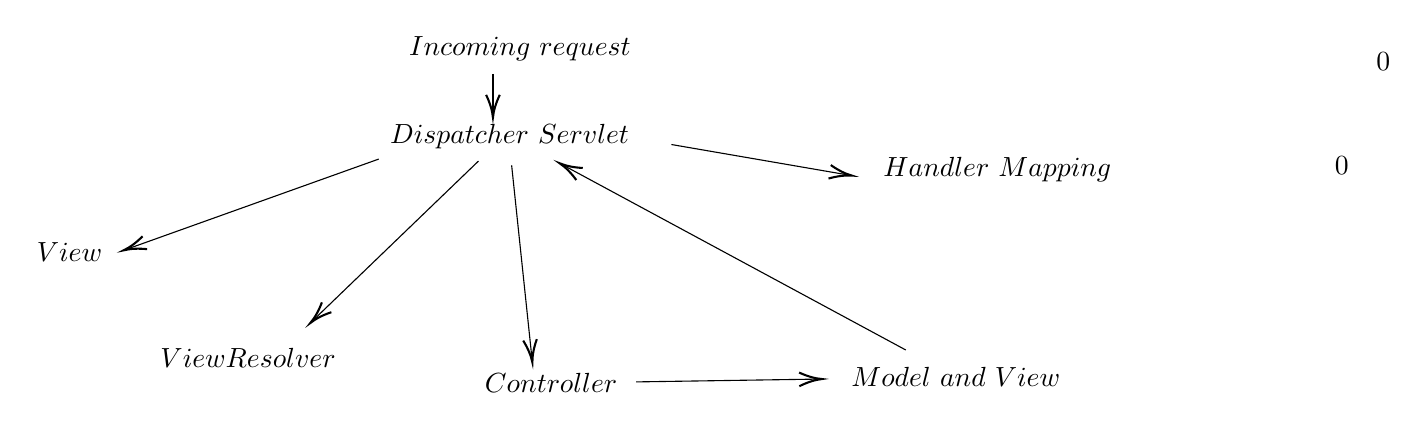
\begin{tikzpicture}[x=0.75pt,y=0.75pt,yscale=-1,xscale=1]
	%uncomment if require: \path (0,235); %set diagram left start at 0, and has height of 235
	
	%Straight Lines [id:da43796635224753366] 
	\draw    (301,71) -- (310.79,164.01) ;
	\draw [shift={(311,166)}, rotate = 263.99] [color={rgb, 255:red, 0; green, 0; blue, 0 }  ][line width=0.75]    (10.93,-3.29) .. controls (6.95,-1.4) and (3.31,-0.3) .. (0,0) .. controls (3.31,0.3) and (6.95,1.4) .. (10.93,3.29)   ;
	%Straight Lines [id:da8543300973373011] 
	\draw    (285,69) -- (205.44,145.61) ;
	\draw [shift={(204,147)}, rotate = 316.08000000000004] [color={rgb, 255:red, 0; green, 0; blue, 0 }  ][line width=0.75]    (10.93,-3.29) .. controls (6.95,-1.4) and (3.31,-0.3) .. (0,0) .. controls (3.31,0.3) and (6.95,1.4) .. (10.93,3.29)   ;
	%Straight Lines [id:da26721417437109896] 
	\draw    (237,68) -- (115.88,111.33) ;
	\draw [shift={(114,112)}, rotate = 340.32] [color={rgb, 255:red, 0; green, 0; blue, 0 }  ][line width=0.75]    (10.93,-3.29) .. controls (6.95,-1.4) and (3.31,-0.3) .. (0,0) .. controls (3.31,0.3) and (6.95,1.4) .. (10.93,3.29)   ;
	%Straight Lines [id:da24273477514405806] 
	\draw    (378,61) -- (463.03,75.66) ;
	\draw [shift={(465,76)}, rotate = 189.78] [color={rgb, 255:red, 0; green, 0; blue, 0 }  ][line width=0.75]    (10.93,-3.29) .. controls (6.95,-1.4) and (3.31,-0.3) .. (0,0) .. controls (3.31,0.3) and (6.95,1.4) .. (10.93,3.29)   ;
	%Straight Lines [id:da4809109559432261] 
	\draw    (292,27) -- (292,46) ;
	\draw [shift={(292,48)}, rotate = 270] [color={rgb, 255:red, 0; green, 0; blue, 0 }  ][line width=0.75]    (10.93,-3.29) .. controls (6.95,-1.4) and (3.31,-0.3) .. (0,0) .. controls (3.31,0.3) and (6.95,1.4) .. (10.93,3.29)   ;
	
	% Text Node
	\draw (300,57) node    {$\text{Dispatcher\ Servlet}$};
	% Text Node
	\draw (515,173) node    {$\text{Model\ and\ View}$};
	% Text Node
	\draw (320,176) node    {$\text{Controller}$};
	% Text Node
	\draw (721,21) node    {$0$};
	% Text Node
	\draw (701,71) node    {$0$};
	% Text Node
	\draw (174,164) node    {$\text{ViewResolver}$};
	% Text Node
	\draw (88,113) node    {$\text{View}$};
	% Text Node
	\draw (535,73) node    {$\text{Handler\ Mapping}$};
	% Text Node
	\draw (305,15) node    {$\text{Incoming\ request}$};
	% Connection
	\draw    (325.85,70.95) -- (490.91,160) ;
	\draw [shift={(324.09,70)}, rotate = 28.35] [color={rgb, 255:red, 0; green, 0; blue, 0 }  ][line width=0.75]    (10.93,-3.29) .. controls (6.95,-1.4) and (3.31,-0.3) .. (0,0) .. controls (3.31,0.3) and (6.95,1.4) .. (10.93,3.29)   ;
	% Connection
	\draw    (448.5,174.02) -- (361,175.37) ;
	\draw [shift={(450.5,173.99)}, rotate = 179.12] [color={rgb, 255:red, 0; green, 0; blue, 0 }  ][line width=0.75]    (10.93,-3.29) .. controls (6.95,-1.4) and (3.31,-0.3) .. (0,0) .. controls (3.31,0.3) and (6.95,1.4) .. (10.93,3.29)   ;
	
\end{tikzpicture}
As displayed in the figure, all the incoming requests are intercepted by the DispatcherServlet that works as the front controller.
The DispatcherServlet gets an entry of handler mapping from the XML file and forwards the request to the controller.
The controller returns an object of ModelAndView.
The DispatcherServlet checks the entry of view resolver in the XML file and invokes the specified view component.

Using Spring MVC comes with numerous advantages. It allows for separation of roles, where the model object, controller, command object, view resolver, DispatcherServlet, validator, etc. can be fulfilled by a specialized object. It uses light-weight servlet container to develop and deploy your application.
It provides a robust configuration for both framework and application classes that includes easy referencing across contexts, such as from web controllers to business objects and validators.
The Spring MVC also facilitates fast and parallel development.
It promotes reusable business code by using the existing business objects instead of creating new ones.
Test of JavaBean classes enables injection of test data using the setter methods, which allows for easier testing.
Flexible Mappings provide the specific annotations that easily redirect the page.
Overall Spring is a powerful tool used by numerous companies and developers around the world.



In this project, Spring has been used to facilitate communication between frontend interface and compiler instances. The REPL is implemented on the server-side as a REST API endpoint. 
\begin{lstlisting}
@PostMapping("/repl")
public ReplResponse repl(HttpSession httpSession, 
    @RequestBody String line)
\end{lstlisting}
Every user has their own instance of REPL
\begin{lstlisting}
Repl repl = (Repl) httpSession.getAttribute("repl");
\end{lstlisting}
which holds a reference to the compiler and a set of built-in commands
\begin{lstlisting}
 public static class Repl {
    private static class CmdMeta<Result> {
        final ReplCommand<Result> cmd;
        final String help;
        final String template;
        
        private CmdMeta(ReplCommand<Result> cmd, 
               String help, String template) {
            this.cmd = cmd;
            this.help = help;
            this.template = template;
        }
    }
     
    HashMap<String, Repl.CmdMeta<String>> commands;
    OptimisedHashLexTransducer compiler;
}
\end{lstlisting}
whenever user types some command on the REPL console
\begin{lstlisting}
:cmd arg1 arg2 arg3
\end{lstlisting}
it gets parsed as
\begin{lstlisting}
String firstWord = "cmd";
String remaining = "arg1 arg2 arg3";
\end{lstlisting}
and then the appropriate command implementation is looked up in the map
\begin{lstlisting}
final Repl.CmdMeta<String> cmd = commands.get(firstWord);
return cmd.cmd.run(httpSession, compiler, log, debug, remaining);
\end{lstlisting}
The rest controller contains implementations of many such commands
\begin{lstlisting}
public static final ReplCommand<String> REPL_LIST = ...
public static final ReplCommand<String> REPL_EVAL = ...
public static final ReplCommand<String> REPL_RUN = ...
public static final ReplCommand<String> REPL_EXPORT = ..
public static final ReplCommand<String> REPL_IS_DETERMINISTIC = ...
public static final ReplCommand<String> REPL_LIST_PIPES = ...
public static final ReplCommand<String> REPL_EQUAL = ...
public static final ReplCommand<String> REPL_RAND_SAMPLE = ...
public static final ReplCommand<String> REPL_CLEAR = ...
public static final ReplCommand<String> REPL_UNSET = ...
public static final ReplCommand<String> REPL_RESET = ...
public static final ReplCommand<String> REPL_LOAD = ...
public static final ReplCommand<String> REPL_VIS = ...
\end{lstlisting}
All of those definitions above are lambda expressions that use library functions
of the compiler. The parameters taken by those lambda expressions are as follows
\begin{lstlisting}
public interface ReplCommand<Result> {
    Result run(
        HttpSession httpSession, 
        OptimisedHashLexTransducer compiler, 
        Consumer<String> log, 
        Consumer<String> debug, 
        String args) throws Exception;
}
\end{lstlisting}
As an example, consider the command 
\begin{lstlisting}
:eval f 'abc'
\end{lstlisting}
which evaluates transducer     exttt{f} for input string     exttt{'abc'}. 
On the frontend JavaScript will perform REST query
\begin{lstlisting}
const response = await fetch('repl', {
     method: 'POST',
     body: ":eval f 'abc'"
})
\end{lstlisting}
which will be received by server
\begin{lstlisting}
@PostMapping("/repl")
public ReplResponse repl(HttpSession httpSession, 
        @RequestBody String line) {
    Repl repl = (Repl) httpSession.getAttribute("repl");
    final String result = repl.run(
        httpSession, 
        line, // ":eval f 'abc'"
        s -> out.append(s).append('\n'), // console output
        s -> { } // debug logs are not displayed
    );
    ...
}
\end{lstlisting}
and the     exttt{repl.run} method will query the appropriate implementation to call for
the     exttt{:eval} command.
\begin{lstlisting}     
final String firstWord = "eval";
final String remaining = "f 'abc'";
final Repl.CmdMeta<String> cmd = commands.get(firstWord);
return cmd.cmd.run(httpSession, compiler, log, debug, remaining);
\end{lstlisting}
This in turn will trigger the following lambda function
\begin{lstlisting}
ReplCommand<String> REPL_EVAL = 
        (httpSession, compiler, logs, debug, args) -> {
    String[] parts = args.split("\\s+", 2); // f 'abc'
    String name = parts[0]; // f
    String input = parts[1]; // 'abc'
    G transducer = compiler.getTransducer(name);
    String output = compiler.specs.evaluate(transducer, input);
    return output == null ? "No match!" : output;
};
\end{lstlisting}
The output is sent back to JavaScript in form of JSON
\begin{lstlisting}
const replResult = JSON.parse(await response.text())
\end{lstlisting}
Remaining commands are implemented in a similar way.

Several of the functions may require access to HTTP session. In particular it's worth analysing the     exttt{:load} command. It's purpose is to emulate the process of loading source code from file. Whenever user types some code in the editor, it needs to be transported to server, then parsed and compiled. All the defined transducers results need to be saved for later use. The simplest way of achieving this, would be by extending the REST API as
\begin{lstlisting}
class ReplInput{
     String command;
     String editorContent;
}
public ReplResponse repl(
    HttpSession httpSession, 
    @RequestBody ReplInput)
\end{lstlisting}
and query it using
\begin{lstlisting}
const response = await fetch('repl', {
    method: 'POST',
    body: {
        command: replCommand,
        editorContent: editor.getValue()
    }
})
\end{lstlisting}
The downside of such solution is that the editor content could become large and sending it would require more internet bandwidth and time. Often user only wants to execute simple short REPL commands that do not require sending the entire code. Sometimes the code might be required but resending it might be omitted as long as user has not modified it. Hence the process of uploading code to the server has been delegated to a separate REST call.
\begin{lstlisting}
const response = await fetch('upload_code', {
     method: 'POST',
     body: code
})
\end{lstlisting}
The code is then stored in HTTP session, so the REST endpoint has a very simple implementation
\begin{lstlisting}
@PostMapping("/upload_code")
public void uploadCode(HttpSession httpSession, 
        @RequestBody String text) {
    httpSession.setAttribute("code", text);
}
\end{lstlisting}


Aside from the editor and REPL there is one more window on the webpage. It is dedicated for tutorial and short documentation.  While it does not enhance the functionality of the website per se, it plays an important role. The Solomonoff compiler is a very niche and specialised tool. There are no similar tools and any user coming to the website is not expected to be familiar with its usage. The primary purpose of the website is not to be a replacement for user's IDE and terminal. Instead it serves as an all-in-one introductory tutorial, interactive playground and a marketing campaign. We want to make the learning materials easily accessible and abundant. Building a strong community is the back-bone of every open-source project. 

\section{Design}


The frontend technologies used for designing our website are based on Bootstrap  \cite{bootstrap}. It is an HTML, CSS \& JS Library that focuses on simplifying the development of informative web pages (as opposed to web apps). The primary purpose of adding it to a web project is to apply Bootstrap's choices of color, size, font and layout to that project. As such, the primary factor is whether the developers in charge find those choices to their liking. Once added to a project, Bootstrap provides basic style definitions for all HTML elements. The result is a uniform appearance for prose, tables and form elements across web browsers. In addition, developers can take advantage of CSS classes defined in Bootstrap to further customize the appearance of their contents. For example, Bootstrap has provisioned for light- and dark-colored tables, page headings, more prominent pull quotes, and text with a highlight.
Bootstrap also comes with several JavaScript components in the form of jQuery plugins. They provide additional user interface elements such as dialog boxes, tooltips, and carousels. Each Bootstrap component consists of an HTML structure, CSS declarations, and in some cases accompanying JavaScript code. They also extend the functionality of some existing interface elements, including for example an auto-complete function for input fields.
The most prominent components of Bootstrap are its layout components, as they affect an entire web page. The basic layout component is called "Container", as every other element in the page is placed in it. Developers can choose between a fixed-width container and a fluid-width container. While the latter always fills the width of the web page, the former uses one of the four predefined fixed widths, depending on the size of the screen showing the page:
\begin{itemize}
	\item Smaller than 576 pixels
	\item 576–768 pixels
	\item 768–992 pixels
	\item 992–1200 pixels
	\item Larger than 1200 pixels
\end{itemize}
Once a container is in place, other Bootstrap layout components implement a CSS Flexbox layout through defining rows and columns.
A precompiled version of Bootstrap is available in the form of one CSS file and three JavaScript files that can be readily added to any project. The raw form of Bootstrap, however, enables developers to implement further customization and size optimizations. This raw form is modular, meaning that the developer can remove unneeded components, apply a theme and modify the uncompiled Sass files.

Below is an example of navigation bar created with help of Bootstraps \texttt{nav} classes.
\begin{center}
	\includegraphics[scale=0.7]{navbar.png}
\end{center}
or responsive panes made with \texttt{flex}, \texttt{row} and \texttt{column} classes
\begin{center}
	\includegraphics[scale=0.4]{panes.png}
\end{center}

Our website has seen numerous design changes. Since the beginning we knew there must be a way to interact with the code but the exact best way of presenting it to the user was not so self-evident. There exist numerous different approaches that are highly dependent on the language. For example the online  Java  compiler consists of only two windows - one for code and one for compiler output.
\begin{center}
\includegraphics[scale=0.3]{java.png}
\end{center}
Java does not have REPL, hence there is no need to implement console input.
A slightly different approach has been taken by Haskell mode for emacs. 
\begin{center}
     \includegraphics[scale=0.45]{haskell.png}
\end{center}
Here it is indeed possible to evaluate smaller snippets of code in the right window, while the left one is solely dedicated to editing local files that can be saved persistently. This is the approach that we settled for in our online playground for Solomonoff. 
\begin{center}
     \includegraphics[scale=0.3]{web8.png}
\end{center}
Before reaching such final version we have experimented with another approach that seemed more natural for regular expressions. Here is an example of a similar website that evaluates UNIX regexes.
\begin{center}
     \includegraphics[scale=0.65]{regex.png}
\end{center}
Initially we tried to mimic such approach with some modifications. Solomonoff is much more complex than UNIX regexes. It allows variables, functions, comments and the overall code could consist of multiple lines. Hence a dedicated multiline editor window was required like in case of Java or Haskell.
\begin{center}
     \includegraphics[scale=0.2]{web3.png}
\end{center}
The upper left window was dedicated to code. The lower left was meant to hold the test input string and the upper right would show the resulting transducer output. Such an approach seemed perfect at the beginning, when Solomonoff was still in early development. Over time, the language became increasingly complex. Several features were added that allowed for visualizing graphs of automata, sampling their languages, testing their formal properties and querying more complex information about them. The interface couldn't keep up with the full range of possibilities offered by he compiler. Hence, we decided to scrap the idea with two input-output windows and tried to emulate console-like REPL instead. The first version looked as follows
\begin{center}
     \includegraphics[scale=0.2]{web6.png}
\end{center}
It was at this point when we first tried to add a window for documentation. A great source of inspiration was the Alt-Ergo online playground. It comes with many helpful examples, which can be automatically copied to the editor upon clicking on them.
\begin{center}
     \includegraphics[scale=0.3]{alt-ergo.png}
\end{center}
Later we extended this idea to a full tutorial with explanations, rather than a simple list of copyable examples. 

\section{Ace editor}

At the same time as the layout of page evolved, we also actively developed the editor itself. While initially we used a simple HTML textarea element, we soon replaced it with the Ace editor. It allowed for integrating many additional features such as syntax highlighting, auto-suggestions, code snippets and marking errors. The core component of working with Ace was the necessity of developing our own syntax highlighting. All the previously mentioned come out-of-the box for existing languages, like JavaScript, C and Python. The matters get much more complicated, when one attempts to define their custom language. Ace documentation for syntax developers tends to be rather sparse. 

There exists a common framework followed by most syntax highlighters. Their configuration consists of two main components - the highlighting rules and the styling rules. The former consist of a set of regular expressions. Any region matched by a certain expression is marked with a list of styles. Then each style decides about the colour. Many existing text editors come with their own syntax highlighter and the required configurations may differ, albeit each format could be automatically converted into any other. 

By using the Iro editor, developer can develop only a single set of rules and then have them automatically converted to any other syntax highlighter. This includes support for Ace, SublimeText, TextMate and Atom. Most of the other editors, like Intellij, Eclipse, Notepad++ etc. use one of the above standards. 

The general format of Iro is as follows
\begin{lstlisting}

styles [] {
     
     .comment : style {
          color                 = #688557
          italic                = true
          ace_scope             = comment
          textmate_scope        = comment
          pygments_scope        = Comment
     }
 
}

main : context {
     
     : pattern {
          regex          \= (//.*)
          styles []       = .comment;
     }
 
}
\end{lstlisting}
each pattern matches some fragment of code and assigns a style to it. Then the style defines colour and scope. The scope is later used as a hint for various other tools that rely on syntax recognition. The colours themselves are also a mere hint. The end user might use an editor that supports various colour palettes. In particular many editors come with optional dark and light theme. Depending on user's choice, our colouring might be overriden. Hence the assigned scope is more important than the colour hint.

Most of the language grammars are context-free and cannot be recognized with a simple regular expression. Hence syntax highlighters allow for using stacks. A good example of this are the block comments. The regular expressions that apply outside of comments should not apply inside them. Iro allows developer to manipulate the stack using push and pop command.
\begin{lstlisting}
: inline_push {
     regex          \= (/\*)
     styles []       = .comment;
     default_style   = .comment
     : pop {
          regex       \= (\*/)
          styles []    = .comment;
     }
}
\end{lstlisting}
Solomonoff's syntax highlighter uses stack to correctly recognize comments and string literals enclosed in quotes and angle brackets. The rest of syntax highlighter is fairly simple and only matches key characters, such as equal signs, brackets, Kleene stars and union vertical pipes as well as variable identifiers.

After the syntax highlighter was developed, Iro automatically generated necessary Ace files. All those configurations are written JavaScript. In order to make them work, it's necessary to clone Ace's repository and compile the custom syntax along with the rest of sources. The compiled project needs to be hosted on website along with remaining JavaScript files. The Ace editor can be initialized using the following lines
\begin{lstlisting}
var editor = ace.edit("editor");
editor.session.setMode("ace/mode/mealy");
\end{lstlisting}
where     exttt{mealy} is the name of our custom syntax.
The editor has been styled using monokai theme
\begin{lstlisting}
editor.setTheme("ace/theme/monokai");
\end{lstlisting}
because its dark palette of colours gives the website a sharp and modern look. The dark theme is preferred by most users and is very popular nowadays. Moreover it's more relaxing to look at and doesn't irritate the eye \cite{syntax_highlighter}. This point is especially important, because Solomonoff is targetted at tech-oriented audiences, so there is a good chance that our users will spend many hours looking at the editor. 

Solomonoff comes with several built-in functions. To make the interface more intuitive and ergonomic the editor needs to provide auto-suggestions with the full range available functions. Below is a list presenting some of the more important options.
\begin{lstlisting}
editor.setOptions({
     enableBasicAutocompletion: [{
          getCompletions: (editor, session, pos,
           prefix, callback) => {
               callback(null, [{
                    name: 'subtract[',
                    value: 'subtract[]',
                    score: 1,
                    meta: 'difference of two languages'
               },
               {
                    name: 'rpni!(',
                    value: 'rpni!()',
                    score: 1,
                    meta: 'RPNI inference algorithm'
               },
               {
                    name: 'rpni_mealy!(',
                    value: 'rpni_mealy!()',
                    score: 1,
                    meta: 'RPNI for Mealy machiens'
               },
               {
                    name: 'ostia!(',
                    value: 'ostia!()',
                    score: 1,
                    meta: 'OSTIA inference for transducers'
               },
               {
                    name: 'compose[',
                    value: 'compose[]',
                    score: 1,
                    meta: 'transducer composition'
               },
               {
                    name: 'inverse[',
                    value: 'inverse[]',
                    score: 1,
                    meta: 'transducer inversion'
               }
               ]);
          },
     }],
     enableSnippets: true,
     enableLiveAutocompletion: true
});
\end{lstlisting}
The     exttt{value} field is the text that autocompletion will produce when selected. The     exttt{meta} argument provides a short explanation that will be shown to the user. We decided to set     exttt{enableLiveAutocompletion} so that the dropdown box with all available functions will automatically show up as soon as the user starts typing. Some less experienced users might not be aware that the suggestions can be triggered manually by pressing     exttt{CTRL+SPACE}. The downside is that in some contexts the autosuggestion will pop up  despite not being necessary. This could irritate some users. Perhaps the best approach would be to make the auto-suggestions configurable. A user could set the editor properties according to their own liking. The only problem was that adding user customizations would increase the complexity of final product. Our goal was not to create a fully functioning IDE. The website is meant to work only as a showcase. Hence the final decision was to make the website as friendly to the newcomers as possible even at the cost of making the experienced users less comfortable. The general consensus was that users that like our product will quickly download the compiler locally and use it in conjunction with their own editor of choice. 

Initially, the Ace  was only used in the main editor window. The REPL console would be made of two text areas, one serving as editable input line and the other for console output, which was permanently set as non-editable. By design, the REPL commands could only be used in console and placing them in the main editor would only result in syntax errors. For instance
\begin{lstlisting}
:eval f 'input'
\end{lstlisting}
would only work in REPL, despite not being a valid Solomonoff code per se. As auto-suggestions were added, it became apparent that showing  REPL commands tin main editor would be very misleading
\begin{lstlisting}
editor.setOptions({
     enableBasicAutocompletion: [{
          getCompletions: (editor, session, pos,
          prefix, callback) => {
               callback(null, [
          ... 
               {
                    name: ':eval',
                    value: ':eval',
                    score: 1,
                    meta: 'evaluate transducer'
               }
          ...
               ]);
          },
     }],
     enableSnippets: true,
     enableLiveAutocompletion: true
});
\end{lstlisting}
On the other hand, not showing any hints related to REPL commands would seems like major shortcoming of the online playground. To address this issue it was later decided tha the REPL input line should also use Ace. As a result the website ended up with two instances of Ace editor. Both very similar to each other. The only difference being that auto-suggestions in REPL input would also display REPL commands, whereas the main code editor would not.

Using Ace in REPL input also happened to solve another problem. Every REPL command would have their own format of argument. For example the     exttt{:eval} would take transducer name and then some input string. The visualization only needs transducer name
\begin{lstlisting}
:vis f
\end{lstlisting}
 The most unintuitive is the random sample command which has two possible formats
 \begin{lstlisting}
:rand_sample f of_size 10
 \end{lstlisting}
and
 \begin{lstlisting}
:rand_sample f of_length 10
\end{lstlisting}
The former generates 10 random member strings, whereas the latter generates all member strings up to length of 10.
The     exttt{of\_size} and     exttt{of\_length} argument decides, which fo the two modes of generation to use. The initial idea to address this issue was to add user help displayed by the     exttt{:?} command.
\begin{lstlisting}
> :?
:vis [ID]
    Shows graph diagram of automaton
:rand_sample [ID] [of_size/of_length] [NUM]
    Generates random sample of input:output pairs produced 
    by ths transducer
:ls
    Lists all currently defined transducers
:clear
    Clears REPL console
:run [ID] [STRING]
    Runs pipeline for the given input
:unset [ID]
    Deletes a variable
:is_det [ID]
    Tests whether transducer is deterministic
:eval [ID] [STRING]
    Evaluates transducer on requested input
...
\end{lstlisting}
User could the consult this cheat sheet to determine format of arguments for each command. Such a solution was simple but it certainly didn't make for the most ergonomic user interface. With Ace it became possible to use code snippets instead.
Below are a few examples.
\begin{lstlisting}
getCompletions: (editor, session, pos, prefix, callback) => {
     callback(null, [
     {
          name: ':eval',
          value: ':eval',
          snippet: ':eval ${1:transducer_name} \'${2:input_string}\'',
          score: 1,
          meta: 'evaluate transducer'
     },
     {
          name: ':rand_sample of_size',
          value: ':rand_sample',
          snippet: ':rand_sample ${1:transducer_name} of_size ${2:number}',
          score: 1,
          meta: 'randomly generate sample'
     },
     {
          name: ':rand_sample of_length',
          value: ':rand_sample',
          snippet: ':rand_sample ${1:transducer_name} of_length ${2:number}',
          score: 1,
          meta: 'randomly generate sample'
     },
     ]);
}
\end{lstlisting}
The structure of arguments for each command was intuitively encoded in form
of blanks that need to be filled in each snippet. Each blank is specified using the \texttt{\$\{\}} braces.

\section{WebAssembly}

WebAssembly \cite{webassembly} is a technology 
that provides a new type of code 
that can be run in modern web browsers, 
providing new functionality and significant 
performance improvements. The code 
for WebAssembly is not meant to be 
written by hand, rather it is designed 
to compile efficiently from low-level 
source languages
such as C, C++, 
Rust, and so on.

WebAssembly allows code
 written
  in 
 different languages
 to run in web applications 
 at near natural speed \cite{webassembly_speed,webassembly_speed2,webassembly_speed3}. 
 This is of great importance 
 for the web platform, as 
 it previously could not be done.

Moreover, it's not necessary to know how to create WebAssembly code in order to use it. WebAssembly modules can be imported into a web application (or Node.js), and functions can be exported from them for use via JavaScript. JavaScript frameworks can use WebAssembly modules to gain tremendous performance benefits and new features, while making their functionality readily available to web developers.


The early versions of Solomonoff compiler were written in C. With help of Emscripten it was possible to then port the code to WebAssembly and call every function directly from JavaScript. Such a solution was preferable, because everything worked on client-side and we could host the website free-of-charge on GitHub
Pages. The WASM interface exposed two functions
\begin{lstlisting}
function compile(){
	console.log(input.value)
	Module.ccall('compile',
	'void',
	['string'], 
	[input.value])
}
function runMealy(){
	console.log(output.value)
	var c = Module.ccall('run_global',
	'string',
	['string'], 
	[output.value])
	console.log(c);
	output.value = c;
}
\end{lstlisting}
First one received a string of source code and the other executed defined transducer. 
Emscripten also generated a layer of JavaScript code in
\begin{lstlisting}
<script async type="text/javascript" src="web_mealy_compiler.js"></script>
\end{lstlisting}
that smoothened process of WebAssembly integration.
At that stage, the compiler was simple and such minimalist API was enough. Later a lot of new functionalities were added and the project requirements shifted to Java. Several approaches for compiling Java code to WASM were attempted but with unsatisfying results.

The first framework we attempted to use was JWebAssembly. We successfully compiled and integrated toy projects but as complexity increased, the limitations became more apparent. The project page itself admitted that JWebAssembly is not yet production ready. Parts of Java standard library were missing, exceptions and threads had limited support and any attempts at converting our compiler to WASM resulted in uncountable of errors.

The next library we attempted was CheerpJ. It was the most promising option. The project compiled successfully and could run in browser. The problem was that support for WASM is still at experimental stage and instead CheerpJ generated JavaScript transcription of our code wrapped in heavyweight runtime. The framework is a commercial product and is primarily targeted at porting Swing/JavaFX applications to browser. There was no documentation explaining how to expose JavaScript API or how to call any Java functions programmatically. There was also no way of manually writing HTML and CSS. Instead the produced applications mimicked typical desktop graphical interface. If we chose to use CheerpJ, we'd be forced to write user interface in Java Swing technology.

The last available option was to use TeaVM\  \cite{teavm}. It suffered similar problems to JWebAssembly. Parts of Java standard library were not supported. Parts of compiler code had to be rewritten to use workaround functions. For instance
the
\begin{lstlisting}
X x = hashMap.computeIfAbsent(k,key->new X());
\end{lstlisting}
had to be rewritten as
\begin{lstlisting}
if(hashMap.conatinsKey(k)){
    x = hashMap.get(k);
}else{
    x = new X();
    hashMap.put(k,x);
}
\end{lstlisting}
Another problem was with porting all the libraries and dependencies.
Parts of ANTLR\  \cite{antlr} code could not be compiled and we resorted to cloning the original ANTLR repo and manually rewriting parts of its code. Clever workarounds had to be implemented but in some cases, the code could not work in browser in any form and had to be removed.
After enough modifications, our code compiled successfully.
When ran in browser, the execution time was prohibitively slow and even the simplest tasks could not be completed in a satisfying time.

As a result, we were forced to forego the idea of compiling Java to WASM and switched to using backend instead. Java has long and extensive history of being used as server-side language with plethora of tools and frameworks available - Spring being one of the most popular.

\end{document}
